

 
\section{Experiment}
\textbf{Dataset} Our experiments used two publicly available data sources, the Tongji hospital dataset\cite{yang2020covid} and Brazil's SARS-CoV-2 dataset\cite{soares2020sars} Tongji dataset consists of 349 chest CT-scans of COVID-19 positive and 397 scans of healthy subjects, all low-resolution CT modalities. Brazil's SARS-CoV-2 dataset consists of 2482 samples, 1252 scans of COVID-19-infected patients, and 1230 healthy subjects collected from multiple hospitals in Sao Paulo, Brazil. The datasets are approved by the corresponding ethical committees of each hospital, Public Hospital of Sao Paulo (HSPM), and Tongji Hospital in Wuhan, China. Train and test sets were obtained randomly from the aggregated datasets. Table \ref{table_datadist}, shows data distribution.


\begin{table}[h!]
\centering
\setlength{\tabcolsep}{6pt}
\renewcommand\arraystretch{1.22}
\caption{ \small Data distribution}
\begin{tabular}{| *{5}{c|} }
\hline
Class  & Dataset & Samples & Train & Test
\\   \hline  
\multirow{2}{3em}{COVID}     &Brazil&1252&\multirow{2}{2em}{1451}  &\multirow{2}{2em}{150}  \\
&Tongji&349&&  \\
\hline
\multirow{2}{6em}{Non-COVID}     &Brazil&1230&\multirow{2}{2em}{1477}  &\multirow{2}{2em}{150}  \\
&Tongji&397&&  \\
\hline
\end{tabular}
\label{table_datadist} 
\end{table}


\textbf{Preprocessing}
Images were selected as 2D slices in greyscale. Preprocessing included randomly cropping between 0.5 to full size, random horizontal flipping, and intensity normalization. CT-slices were all resized to 224$\times$224 pixels with interpolation. Figure \ref{fig:samplesCTs} shows samples of processed images.
% \quickthings{This looks like you have a bias in your dataset. You should select the normals and abnormals at comparable level in the thorax. All covid are now lower in the body then the non-covid ones.}
% \maybelater{I have changed the picture, hope it's okay now}
\begin{figure}[h!]
 \centering
 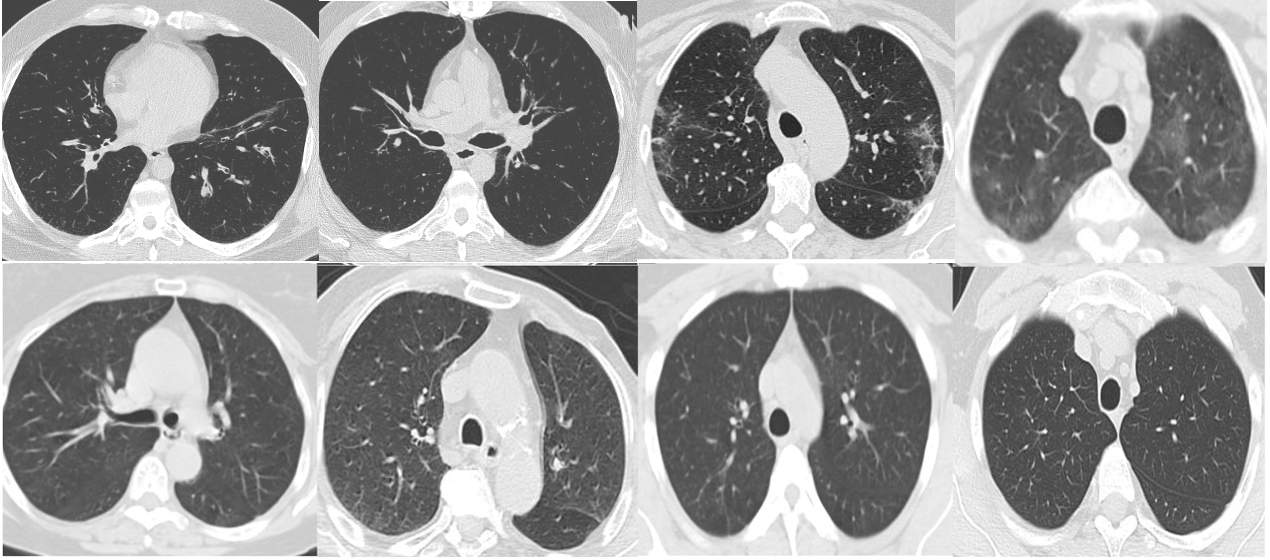
\includegraphics[width=0.45\textwidth]{covidexamples3.png}
 \caption{Sample CT slices of COVID-19 images (top row) and Non-COVID images (bottom row)}
 \label{fig:samplesCTs}
\end{figure}


% normalize = transforms.Normalize(mean=[0,0,0], std=[1,1,1])
% train_transformer = transforms.Compose([
%     transforms.Resize(256),
%     transforms.RandomResizedCrop(224, scale=(0.5, 1.0)),
%     transforms.RandomHorizontalFlip(),
%     transforms.ToTensor(),
%     normalize
% ])

\textbf{Training}
ResNet-18 is used as the backbone deep learning model. ResNet-18 comprises one initial block cascaded to four middle blocks. The initial block is made of convolutional,  batch normalization, ReLU, and pooling layers. Middle blocks have the same layers, connected with straight and skip connections. The model is pre-trained on ImageNet dataset \cite{he2016deep} with a CrossEntropy loss function and learning rate of $0.05$. 
Each federated round consisted of 20 internal epochs for each client and batches of 16 samples in each iteration. For models which use minibatch training, like STWT and FedSGD, a subset of clients is randomly selected. Similar to training, test data was split into mini-batches, and the results were averaged across batches. We performed training with various participating clients and federated rounds to evaluate their effect on final performance. Models were also trained in a centralized, non-federated setting to build a comparison baseline. Figure \ref{fig:distributionsite} shows the data distribution among clients.

\begin{figure}[h!]
 \centering
 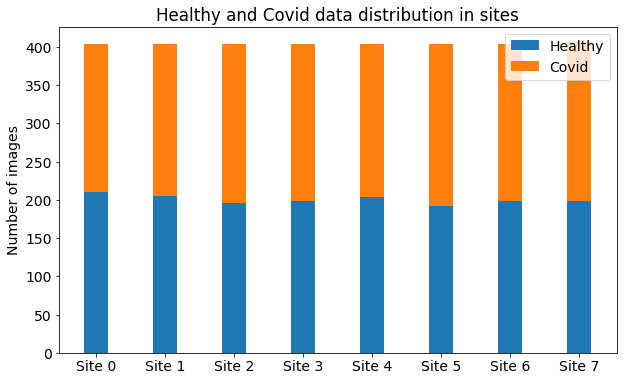
\includegraphics[width=0.7\textwidth]{output.png}
 \caption{Data distribution of each client in the simulated federated setting}
 \label{fig:distributionsite}
\end{figure}
% \abs{Healthy COVID data distirbution per site}

\textbf{Evaluation} 
Standard classification metrics, accuracy, recall, precision, and F1 score, were used as our evaluation criteria. We also evaluated the level of communication, the amount of transferred data in each algorithm, and the computational complexity of the models. 
\label{sec:experiment}
